\section{文献阅读}

\begin{frame}{中科院\ 2020\ 博士\ 冯旭斌}
    \textbf{基于深度学习的光学遥感图像去噪与超分辨率重建算法研究}\\[1cm]

    \begin{itemize}
        \item 光学遥感可用于多领域
        \item 通过硬件提高影像质量成本高
        \item 如何经济, 高效提高光学遥感影像质量很重要
    \end{itemize}
\end{frame}

\begin{frame}{中科院\ 2021\ 硕士\ 熊鹰飞}
    \textbf{基于生成对抗网络的多跨源区域遥感图像超分辨}\\[1cm]

    \begin{itemize}
        \item 土地覆盖, 土地利用需要高分辨率影像
        \item 遥感卫星空间分辨率与重访周期矛盾, 通常使用超分提高分辨率获得高分辨率影像
        \item 相比传统方法, 深度学习GAN更适合影像超分
        \item 本文在SRGAN基础上增强了模型跨区域和传感器迁移能力
    \end{itemize}
    
\end{frame}

\begin{frame}{哈工大\ 2018\ 硕士\ 李鸿飞}
    \textbf{光学遥感图像超分辨率重构方法研究}\\[1cm]
    
    \begin{itemize}
        \item 高分辨率遥感影像在各领域的重要意义
        \item 通过硬件提高影像质量受到工艺水平, 研制难度等因素
        \item 因此从图像处理的方式提高图像分辨率
    \end{itemize}
\end{frame}

\begin{frame}{中科院\ 2017\ 博士\ 赵晓东}
    \textbf{光学遥感影像超分辨率重构算法研究}\\[1cm]
    
    \begin{itemize}
        \item 高分辨率遥感影像在各领域的重要意义
        \item 获取高分辨率影像受到各种因素影响
        \item 超分可在现有成像系统上, 利用图像处理信号处理重构高分辨率影像, 具有一定研究意义
    \end{itemize}
\end{frame}

\begin{frame}{中科院\ 2017\ 博士\ 赵晓东}
    \textbf{光学遥感影像超分辨率重构算法研究}\\[1cm]
    文章在第一章举了如下两个例子:
    \begin{itemize}
        \item 火星探测器Viking获得低分图像超分重建环境
        \item 法国SPOT-5将超分亚像元技术
        \item 军事中提高影像分辨率可提高目标识别率
    \end{itemize}
\end{frame}

\begin{frame}{电子科大\ 2020\ 硕士\ 韦志深}
    \textbf{基于超分辨率重建的遥感影像亚像元目标识别研究}\\[1cm]

    \begin{itemize}
        \item 低分影像无法满足对遥感影像处理要求
        \item 在原有硬件系统条件下, 利用软件技术进行超分
    \end{itemize}
\end{frame}

\begin{frame}{哈工大\ 2020\ 硕士\ 潘梦迪}
    \textbf{基于深度学习的机载遥感图像超分辨率重建}\\[1cm]

    \begin{itemize}
        \item 机载遥感图像受环境影响大且受硬件影像, 分辨率低
        \item 因此要利用超分技术保证图像清晰度
    \end{itemize}
\end{frame}

\begin{frame}{华东理工\ 2019\ 硕士\ 陈敏强}
    \textbf{深度卷积神经网络超分重建技术驱动的卫星遥感影像融合研究}\\[1cm]

    \begin{itemize}
        \item 通过超分, 研究影像融合
        \item 提高影像质量通过硬件和软件
        \item 硬件成本过高, 超分不受硬件系统限制, 前景广阔
    \end{itemize}
\end{frame}

\begin{frame}{中科院\ 2019\ 博士\ 杨蕊}
    \textbf{动态序列遥感图像超分辨率重建技术研究}\\[1cm]

    \begin{quotation}
        图像超分辨重建技术恰好可以用时间分辨率换空间分辨率, 它可以在不改变硬件水平的条件下提高动态序列遥感数据的空间分辨率. 超分辨率重建技术能够充分结合动态序列图像的特点, 在低成本的前提下取得更高质量的遥感图像, 在遥感数据处理领域特别是商业卫星中具有很高的科研价值和商业利益, 因此获得广泛的关注.
    \end{quotation}
\end{frame}

\begin{frame}{西安科技大学\ 2020\ 硕士\ 师珂珂}
    \textbf{遥感图像超分辨率重建算法研究}\\[1cm]

    \begin{quotation}
        提升成像设备硬件条件是获得高分辨率遥感图像最直接有效的方法. 该方法主要分为两种: 一是改进传感器的制作工艺以减小像素尺寸. 然而, 随着像素尺寸的不断减小其获得的光线数量也随之越少, 最终会引入散粒噪声, 从而导致图像质量降低; 二是增加传感器上光敏元件的个数以增大单位面积内像素的数量. 这种做法会导致经济成本的显著增加, 限制了通过硬件方法来得到高分辨率图像技术的发展与应用.
    \end{quotation}
\end{frame}

\begin{frame}{超分其他应用}
    \begin{itemize}
        \item 基于多路卷积神经网络和超分辨率的绿潮提取方法\	赵尊强\ 山东科技大学
        \item 遥感影像超分辨率重建方法研究及其在水域监测中的应用	\ 颜苏东\ 南昌工程学院
        \item 遥感图像超分辨率重建与目标检测方法研究\ 周康\	西安电子科技大学
        \item 	基于超分辨率重建滇中地区土地覆盖遥感分类研究\ 王丽霞\ 云南师范大学
        \item 遥感影像超分辨率制图技术研究---以湖南望城乔口镇为例\ 刘细梅\ 中南大学
        \item 基于图像超分辨率的遥感图像树冠目标检测
    \end{itemize}
\end{frame}

\begin{frame}{超分其他应用}
    \begin{itemize}
        \item 超分辨率重建技术在海域使用疑点疑区监管中的应用
        \item 超像元尺度下的多光谱图像超分辨率洪水淹没制图
    \end{itemize}
\end{frame}
% \begin{frame}{可用哨兵数据空间位置}
%     \small
%     考虑到六幅影像的范围有重叠, 只用其中一组即可
%     \begin{figure}
%         \centering
%         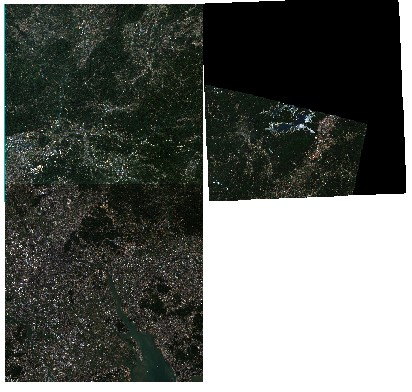
\includegraphics[width=6cm]{pic/pic0115.jpg}
%         \caption{哨兵可用重叠}
%         \label{fig:0109}
%     \end{figure}
% \end{frame}

% \begin{frame}{数据查询}
%     \begin{columns}
%         \column{0.3\textwidth}
%         \begin{itemize}
%             \item \small{对广东区域进行影像检索}
%         \end{itemize}

%         \column{0.7\textwidth}
%         \begin{figure}
%             \centering
%             % Requires \usepackage{graphicx}
%             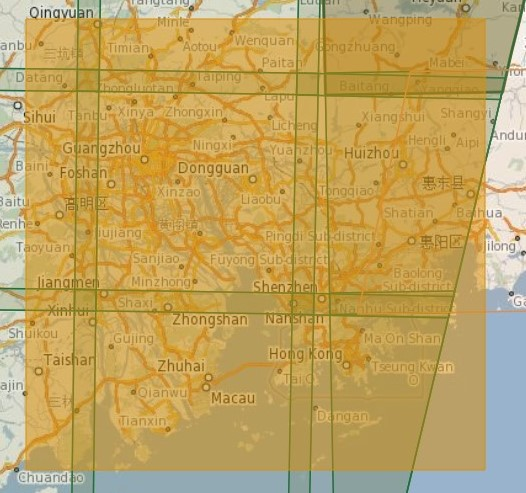
\includegraphics[width=5cm]{pic/pic0101.jpg}
%             \caption{影像查询地区}
%             \label{fig:0101}
%         \end{figure}
%     \end{columns}
% \end{frame}